\section{Giải pháp ước lượng kênh MMSE, LS, và máy học}

\subsection{Ước lượng kênh bằng MMSE}

Phương pháp Minimum Mean Square Error (MMSE) là một trong những phương pháp ước lượng kênh truyền tiên tiến, mang lại độ chính xác cao hơn so với Least Squares (LS) bằng cách sử dụng thông tin thống kê về kênh truyền và nhiễu. 
MMSE không chỉ giảm thiểu sai số giữa kênh ước lượng và kênh thực mà còn tối ưu hóa hiệu suất trong môi trường có nhiễu và fading mạnh. 

\subsubsection{Mục tiêu của ước lượng MMSE}

MMSE dựa trên việc tối thiểu hóa trung bình bình phương sai số (MSE) giữa kênh truyền thực tế và kênh ước lượng. 
Điều này có nghĩa là MMSE không chỉ dựa vào tín hiệu đã nhận mà còn sử dụng thông tin thống kê về kênh truyền và nhiễu, 
từ đó đưa ra ước lượng tốt hơn so với LS. 
Cụ thể, MMSE cố gắng tối thiểu hóa sai số kỳ vọng giữa kênh thực và kênh ước lượng bằng cách tìm ma trận lọc tối ưu.

Dựa trên kênh truyền đã được ước lượng bằng phương pháp LS:
% 
\begin{align*}
    \bm{\hat{H}_p} 
    &= \bm{y_p}\bm{x_p}^H \\
    &= (\bm{H_d}\bm{x_p} + \bm{n})\bm{x_p}^H \\
    &= \bm{H_d}\bm{x_p}\bm{x_p}^H + \bm{n}\bm{x_p}^H \\
    &= \bm{H_d} + \bm{n}\bm{x_p}^H
\end{align*}

Ta tiến hành nhân kênh truyền đã ước lượng LS với một ma trận lọc \( \bm{W} \):

\[
    \bm{\hat{H}} = \bm{W}\bm{\hat{H}_p} 
\]

\begin{figure}[H]
    \centering
    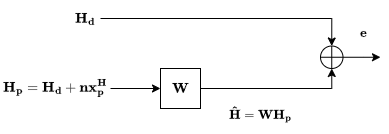
\includegraphics[width=.75\textwidth]{../images/mmse_block_diagram.png}
    \caption{Ước lượng kênh bằng phương pháp MMSE}
\end{figure}

Mục tiêu của phương pháp ước lượng MMSE là tìm ma trận lọc \( \bm{W} \) 
sao cho nó \textbf{giảm thiểu sai số bình phương trung bình} MSE giữa kênh truyền thực tế \( \bm{H_d} \) 
và kênh truyền ước lượng \( \bm{\hat{H}} = \bm{W}\bm{\hat{H}_p} \). 
MSE có thể được định nghĩa qua hàm mất mát (loss function) như sau:

\begin{equation}
    \bm{J(W)} 
    = \bb{E} \left[ \| \bm{e} \|^2 \right]
    = \bb{E} \left[ \| \bm{H_d} - \bm{W}\bm{\hat{H}_p} \|^2 \right]
\end{equation}

Trong đó, \( \bm{e} = \bm{H_d} - \bm{W}\bm{\hat{H}_p} \) là ma trận sai số giữa kênh thực tế và kênh ước lượng.

Để tối thiểu hóa MSE, ta cần tìm \( \bm{W} \) để tối thiểu hàm mất mát. 
Điều này được thực hiện bằng cách giải phương trình tối ưu hóa sau:
%
\begin{equation}
    \bm{W} 
    = \underset{\bm{W}}{\arg \min} \; \bm{J(W)}
    = \underset{\bm{W}}{\arg \min} \; \bb{E} \left[ \| \bm{H_d} - \bm{W}\bm{\hat{H}_p} \|^2 \right]
\end{equation}

\subsubsection{Tìm nghiệm tối ưu của ước lượng MMSE}

Dựa trên nguyên lý trực giao, ta có ma trận sai số \( \bm{e} \) trực giao với \( \bm{\hat{H}} \). 
Hơn nữa, \( \bm{\hat{H}} = \bm{W}\bm{\hat{H}_p} \) với \( \bm{W} \) là ma trận của một phép biến đổi tuyến tính, nên \( \bm{e} \) cũng trực giao với \( \bm{\hat{H}_p} \):

\begin{figure}[H]
    \centering
    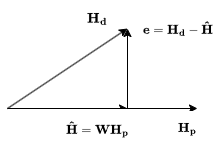
\includegraphics[width=.4\textwidth]{../images/mmse_orthogonal.png}
    \caption{Ma trận sai số \( \bm{e} \) trực giao với \( \bm{\hat{H}_p} \)}
\end{figure}

\begin{align*}
    \bb{E} \left[ \bm{e} \bm{\hat{H}_p}^H \right] 
    &= \bb{E} \left[ (\bm{H_d} - \bm{W}\bm{\hat{H}_p}) \bm{\hat{H}_p}^H \right] \\
    &= \bb{E} \left[ \bm{H_d}\bm{\hat{H}_p}^H - \bm{W}\bm{\hat{H}_p}\bm{\hat{H}_p}^H \right] \\
    &= \bb{E} \left[ \bm{H_d}\bm{\hat{H}_p}^H \right] - \bm{W}\bb{E} \left[ \bm{\hat{H}_p}\bm{\hat{H}_p}^H \right] \\
    &= \bm{R_{dp}} - \bm{W}\bm{R_{pp}} = 0
\end{align*}

Trong đó, \( \bm{R_{dp}} = \bb{E} \left[ \bm{H_d}\bm{\hat{H}_p}^H \right] \) là ma trận tương quan giữa kênh thực và kênh ước lượng, 
và \( \bm{R_{pp}} = \bb{E} \left[ \bm{\hat{H}_p}\bm{\hat{H}_p}^H \right] \) là ma trận tự tương quan của kênh ước lượng tại các vị trí pilot.

Từ đó, ta có:

\[
    \bm{W} = \bm{R_{dp}} \bm{R_{pp}}^{H}
\]

\( \bm{R_{pp}} \) được tính bởi:
% 
\begin{align*}
    \bm{R_{pp}} 
    &= \bb{E} \left[ \bm{\hat{H}_p}\bm{\hat{H}_p}^H \right] \\
    &= \bb{E} \left[ (\bm{H_d} + \bm{n}\bm{x_p}^H)(\bm{H_d} + \bm{n}\bm{x_p}^H)^H \right] \\
    &= \bb{E} \left[ \bm{H_d}\bm{H_d}^H + \bm{H_d}\bm{n}^H\bm{x_p} + \bm{n}\bm{x_p}^H\bm{H_d}^H + \bm{n}\bm{n}^H\bm{x_p}\bm{x_p}^H \right] \\
    &= \bm{R_{dd}} + \sigma_n^2\bm{x_p}\bm{x_p}^H
\end{align*}

Trong đó, \( \bm{R_{dd}} = \bb{E} \left[ \bm{H_d}\bm{H_d}^H \right] \) là ma trận tương quan của kênh thực tế. Thay vào phương trình trên, ta có:

\begin{equation}
    \bm{W} = \bm{R_{dp}} (\bm{R_{dd}} + \sigma_n^2\bm{x_p}\bm{x_p}^H)^{H}
\end{equation}

Phương pháp này dựa vào việc mô tả thống kê của kênh truyền và tín hiệu nhận được. 
Nếu các ma trận tương quan này được ước lượng chính xác, MMSE sẽ cho kết quả ước lượng kênh chính xác hơn đáng kể so với LS.

\subsubsection{Ước lượng kênh tại các vị trí không phải pilot}

Để ước lượng kênh tại các vị trí không phải pilot, phương pháp nội suy có thể được áp dụng. 
Do MMSE đã khai thác thông tin thống kê của kênh, kết quả nội suy thường chính xác hơn so với nội suy từ ước lượng LS.

